%------------------------------------------------------------------------------
\chapter{Additional plots and calculations}
\label{sec:app}
%------------------------------------------------------------------------------
This chapter will give additional calculations and plots which would have interrupted the train of thought unnecessarily in the main part. 
\section{Statistical error for the asymmetry $A(\phi)$}
\allowdisplaybreaks
\label{sec:stat_err}
Let $\tilde{N}^{\parallel/\bot}_i$ be the normalized event yields at bin $\phi_i$. As mentioned in section \ref{sec:meth}, the asymmetry $A_i$ at bin $i$ is then given by
\begin{equation}
	A_i=\frac{\tilde{N}^\bot_i-\tilde{N}^\parallel_i}{p_\gamma^\parallel\tilde{N}^\bot_i+p_\gamma^\bot\tilde{N}^\parallel_i}=\Sigma\cos\left(2\left(\alpha^\parallel-\phi_i\right)\right),
	\label{eq:evyieldasym_app}
\end{equation}
where the event yields are normalized over all $M$ $\phi$-bins $$\tilde{N}^{\parallel/\bot}_i=\frac{N_i^{\parallel/\bot}}{\sum_{j=1}^{M}N_j^{\parallel/\bot}}.$$
 To estimate statistical errors according to \textsc{Gaussian} error propagation, the partial derivatives with respect to $\tilde{N}_i^{\parallel/\bot}$ have to be built:
 \begin{equation}
 	\left(\Delta A_i\right)^2=\left(\frac{\partial A_i}{\partial \tilde{N}^\parallel_i}\Delta \tilde{N}^\parallel_i\right)^2+\left(\frac{\partial A_i}{\partial \tilde{N}^\bot_i}\Delta \tilde{N}^\bot_i\right)^2,
 \end{equation}
where
\begin{align}
	\left(\frac{\partial A_i}{\partial \tilde{N}^{\parallel/\bot}_i}\right)^2&=\left[\frac{\tilde{N}^{\bot/\parallel}_i\left(p_\gamma^\bot+p_\gamma^\parallel\right)}{\left(p_\gamma^\parallel\tilde{N}^{\bot}_i+p_\gamma^\bot\tilde{N}^\parallel_i\right)^2}\right]^2,\\
	&\text{ and with } \tilde{N}_i^{\bot/\parallel}=\tilde{N}_i\\
	\left(\Delta\tilde{N}_i\right)^2&=\left[\frac{\partial}{\partial N_i}\left(\frac{N_i}{\sum_{j}N_j}\right)\cdot\Delta N_i\right]^2+\sum_{j\neq i}\left[\frac{\partial}{\partial N_j}\left(\frac{N_i}{\sum_{j}N_j}\right)\cdot\Delta N_j\right]^2\\
	&=\left[\frac{\sum_{j\neq i} N_j}{\left(\sum_{j} N_j\right)^2}\cdot\Delta N_i\right]^2+\sum_{j\neq i}\left[-1\cdot\frac{N_i}{\left(\sum_{j}N_j\right)^2}\cdot\Delta N_j\right]^2\\
	&=\frac{1}{\left(\sum_{j} N_j\right)^4}\cdot\left[\left(\sum_{j\neq i} N_j \cdot\Delta N_i\right)^2+\sum_{j\neq i}\left(N_i\cdot\Delta N_j\right)^2\right].
\end{align}
One can then further use that $\left(\Delta N_i\right)^2  \approx N_i$. This holds only approximately, since the histograms are filled $N$ times with weights $w_n$ (see chapter \ref{sec:time}), but since the weights are either $w=1$ or $w\ll1$
\begin{equation}
	\Delta N_i=\sqrt{\sum_{n=1}^N w^2}\approx\sqrt{N_i}.
\end{equation}
\newpage
\section{Kinematic variables for each bin}
\label{sec:kinv}
\subsection{Coplanarity}
\begin{figure}[H]
	\centering
	\begin{subfigure}{\linewidth}
		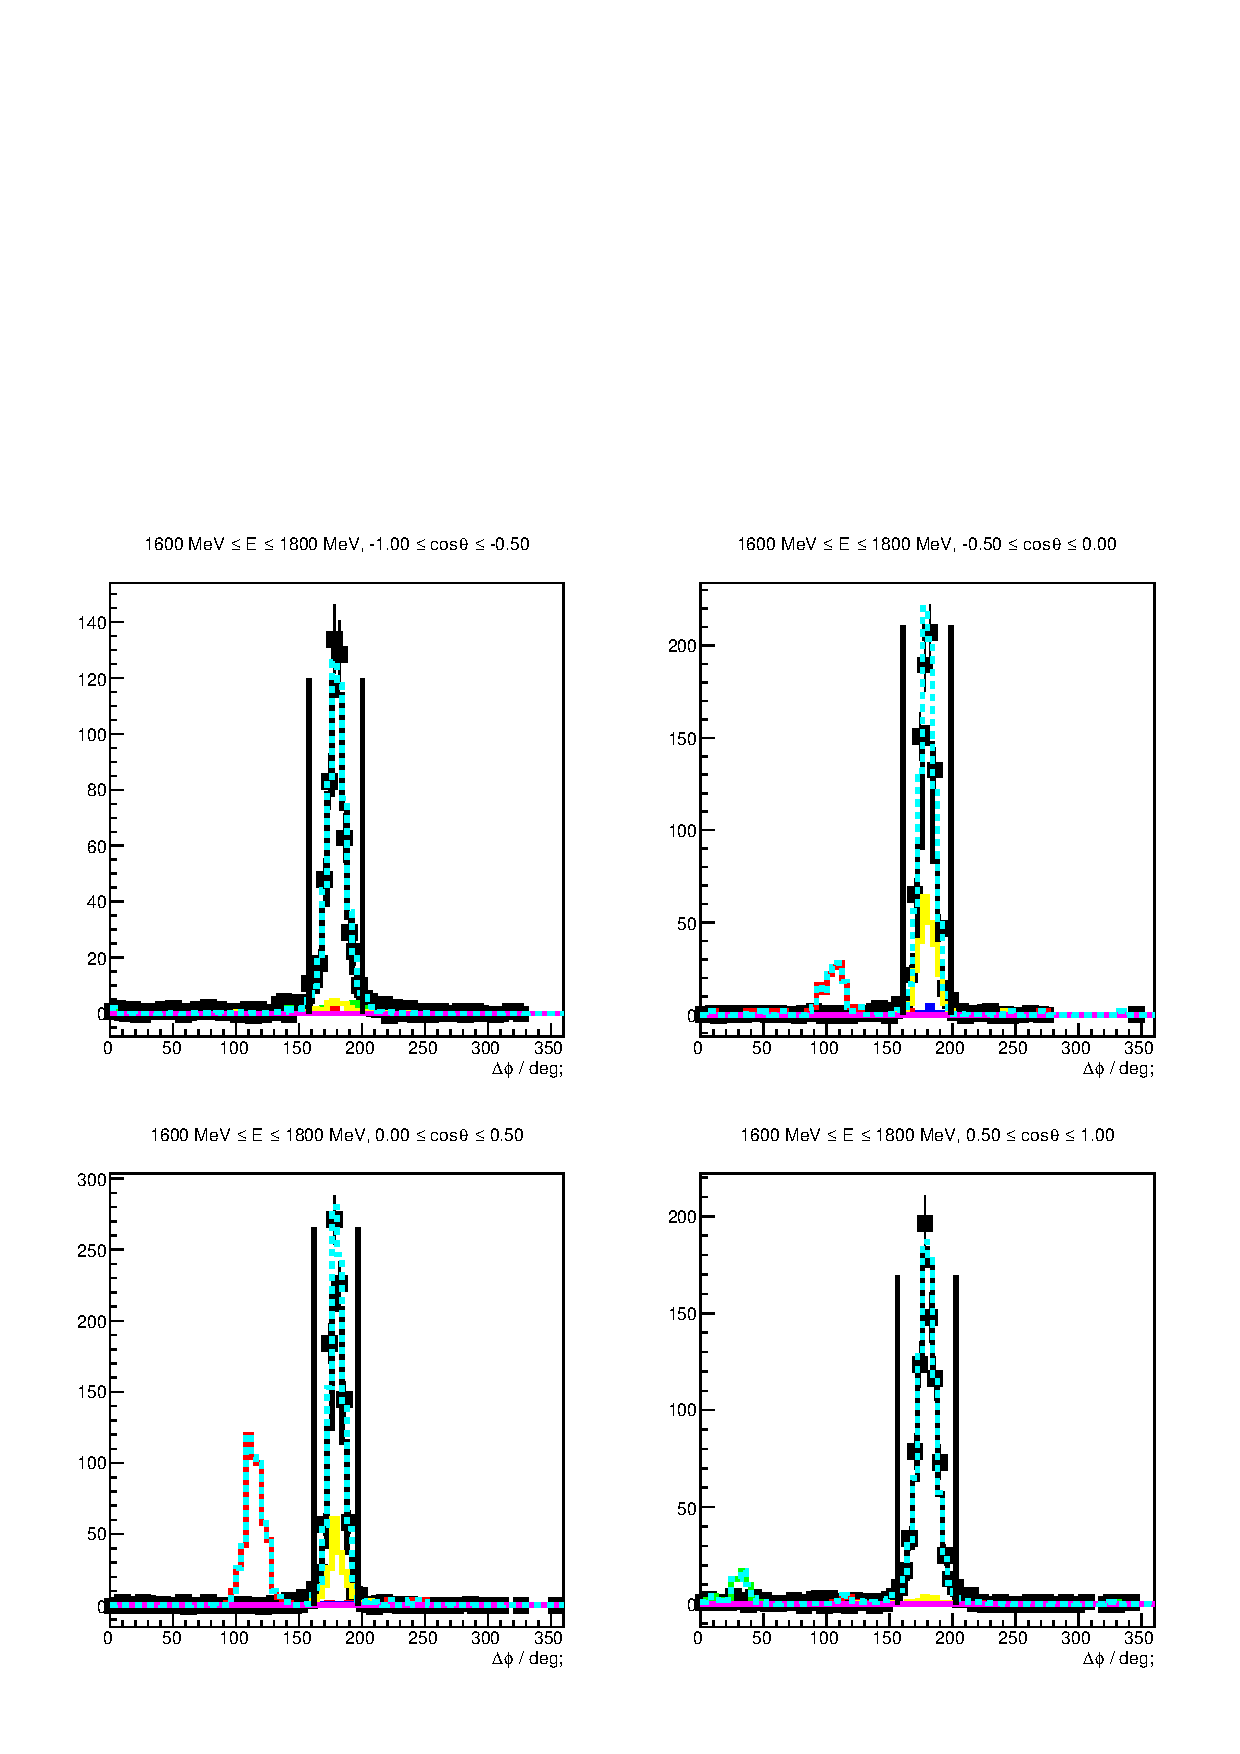
\includegraphics[width=\linewidth]{../figs/hydrogen/bin_cuts/phicut_ebin1.pdf}
		\subcaption{$\SI{1500}{\mega\eV}\leq E_\gamma<\SI{1600}{\mega\eV}$}
	\end{subfigure}

	\begin{subfigure}{\linewidth}
		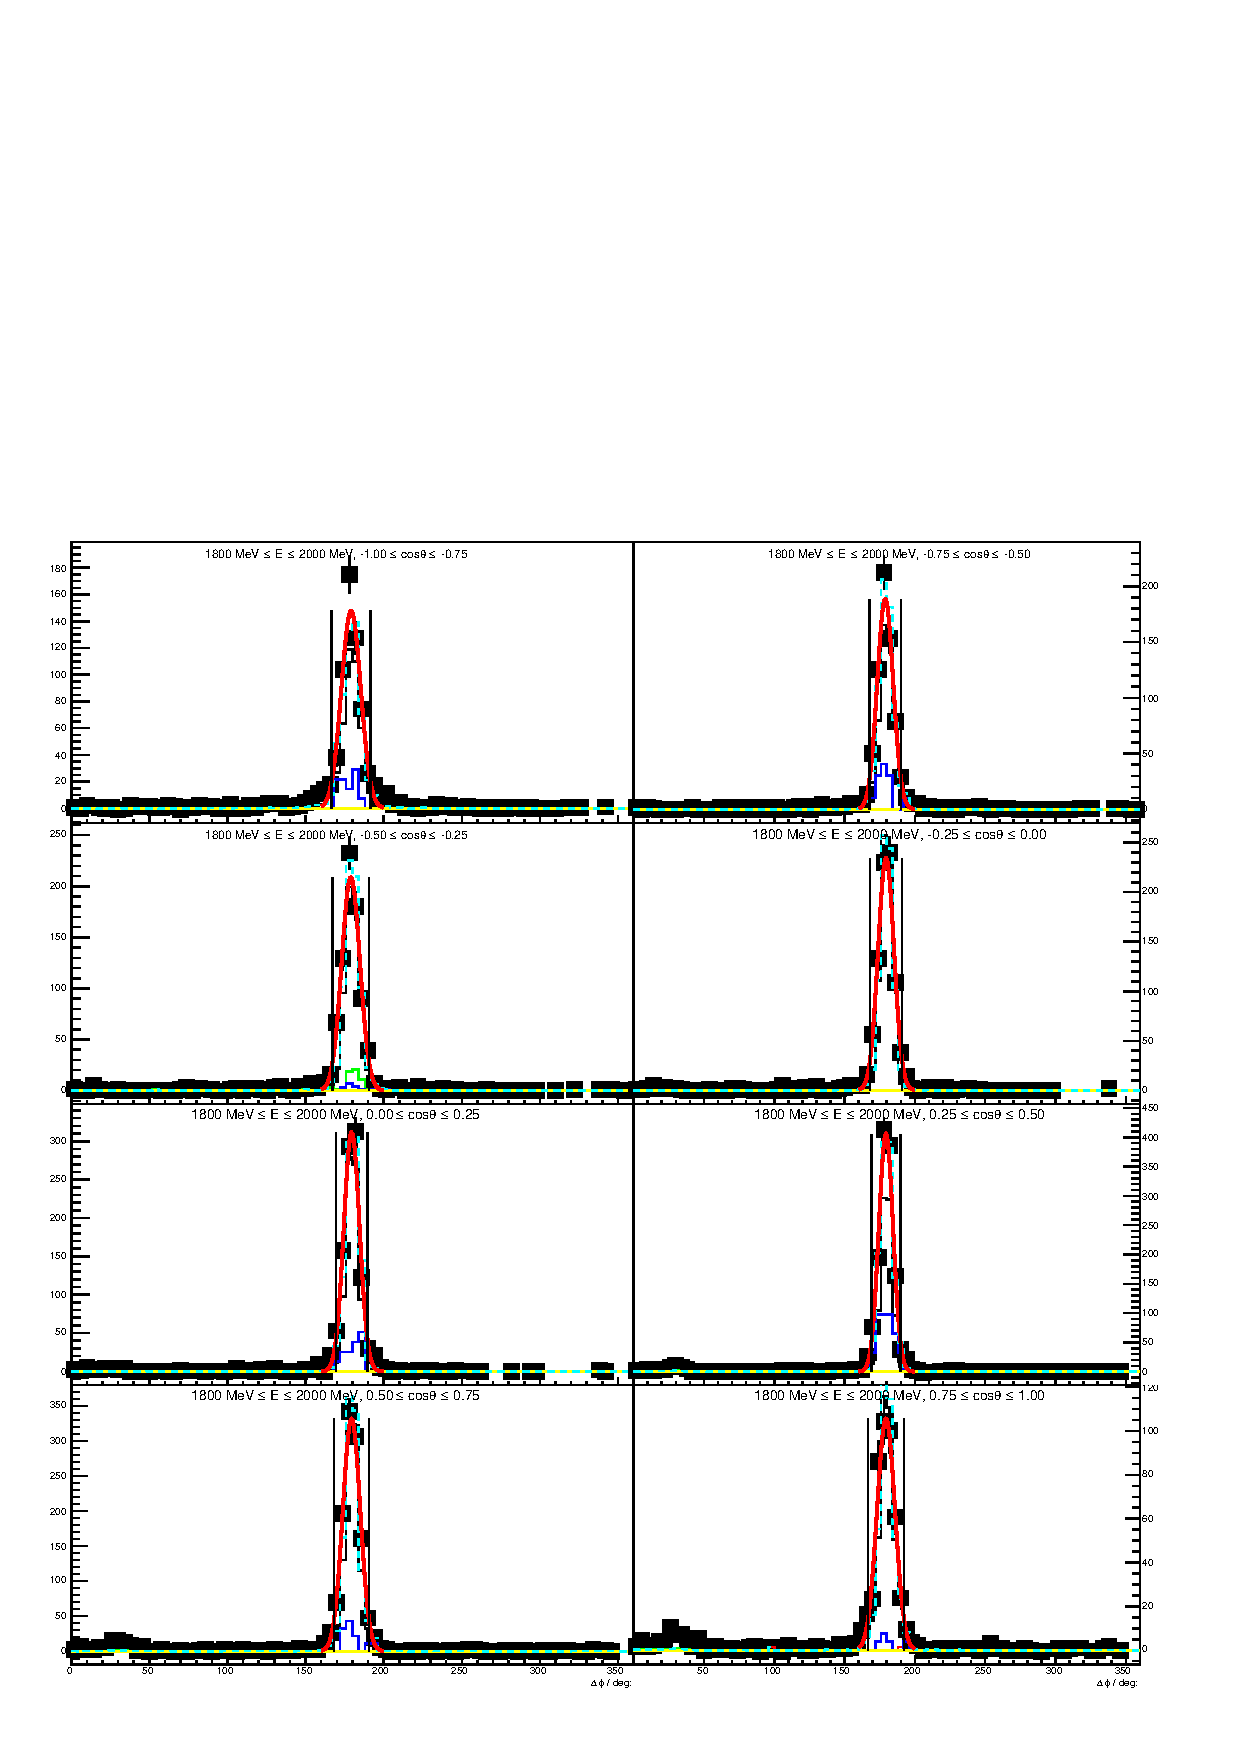
\includegraphics[width=\linewidth]{../figs/hydrogen/bin_cuts/phicut_ebin2.pdf}
		\subcaption{$\SI{1600}{\mega\eV}\leq E_\gamma<\SI{1700}{\mega\eV}$}
	\end{subfigure}
\caption{Coplanarity $\Delta\phi$ for all energy and angular bins. Data points are displayed as open circles, scaled Monte Carlo data belonging to $\eta'$ photoproduction is displayed as solid histogram. The determined cut ranges are indicated by the dashed red lines.}
\end{figure}
\begin{figure}[H]
\ContinuedFloat
	\begin{subfigure}{\linewidth}
		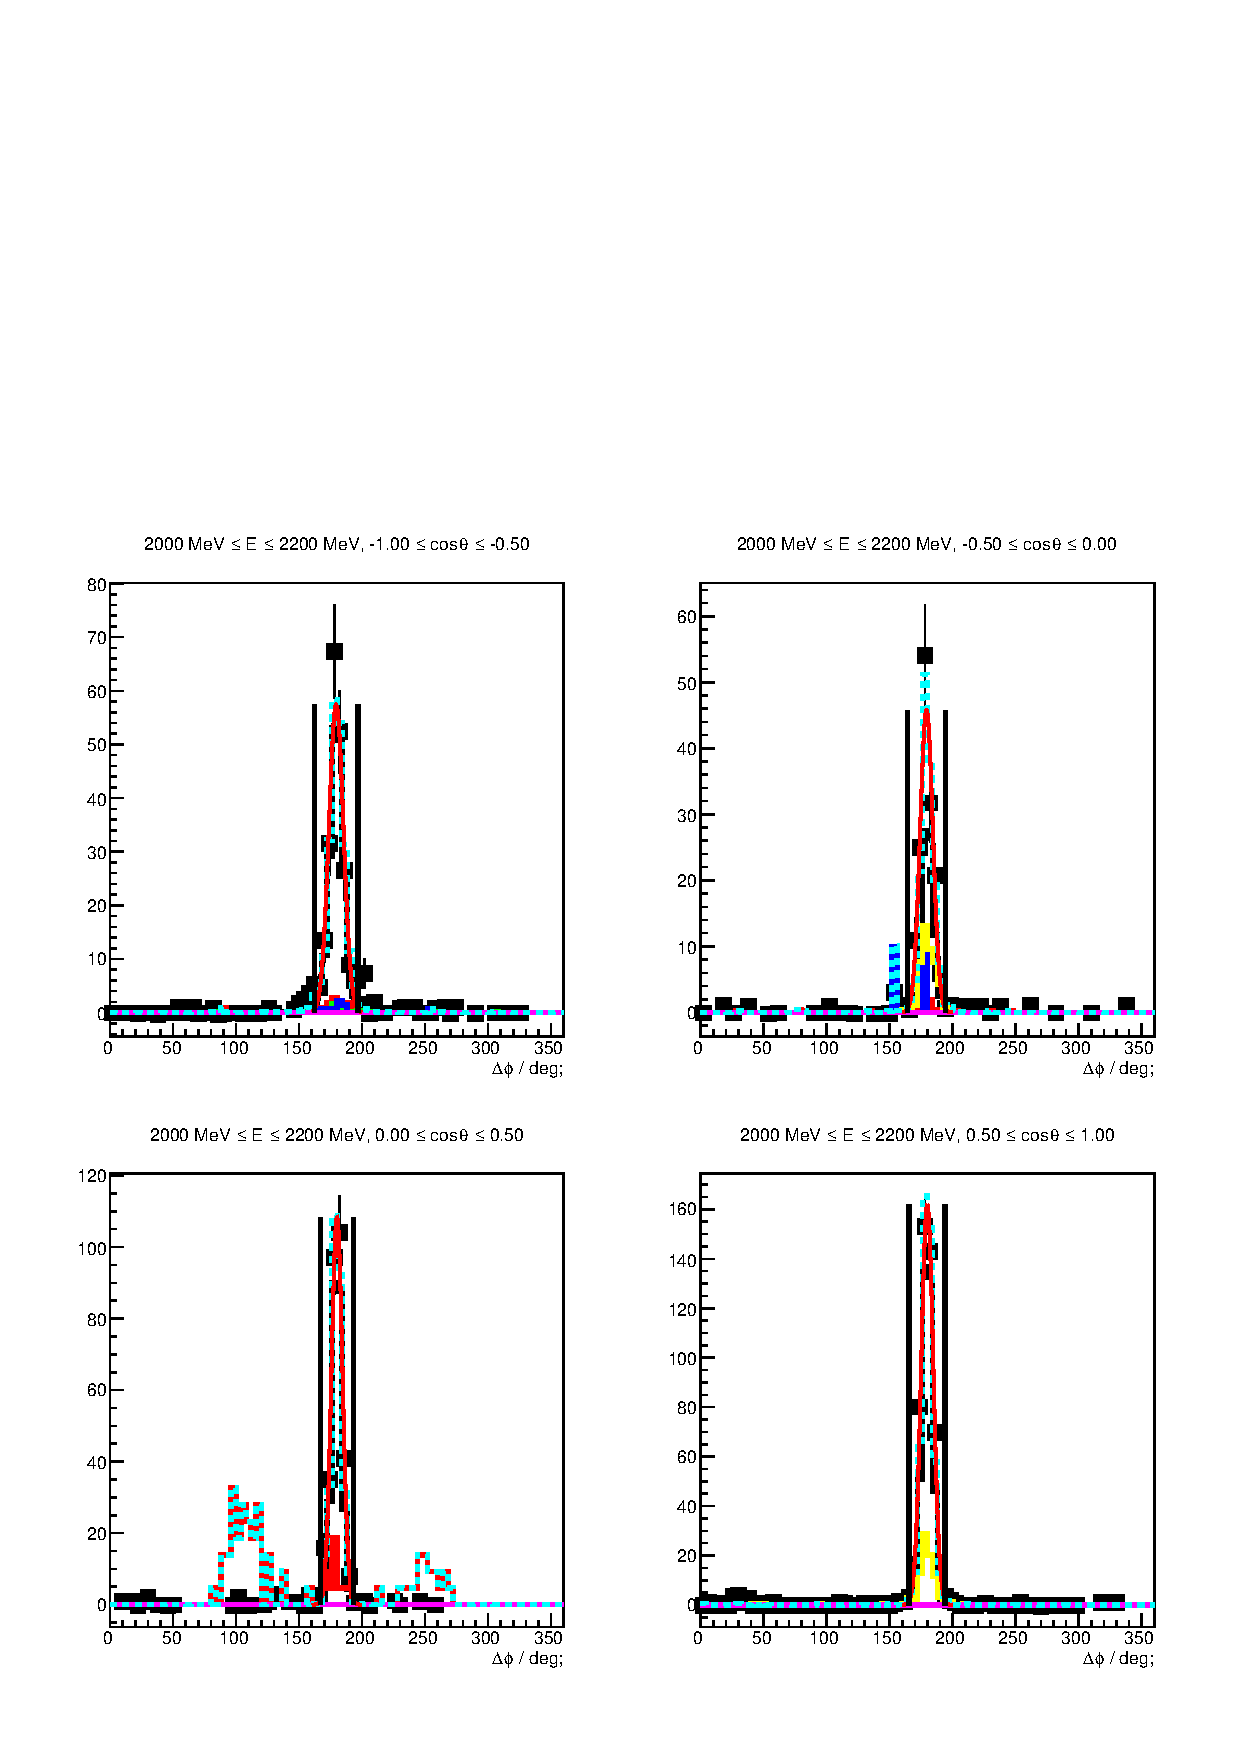
\includegraphics[width=\linewidth]{../figs/hydrogen/bin_cuts/phicut_ebin3.pdf}
		\subcaption{$\SI{1700}{\mega\eV}\leq E_\gamma<\SI{1800}{\mega\eV}$}
	\end{subfigure}
\caption{Coplanarity $\Delta\phi$ for all energy and angular bins. Data points are displayed as open circles, scaled Monte Carlo data belonging to $\eta'$ photoproduction is displayed as solid histogram. The determined cut ranges are indicated by the dashed red lines.}
\label{fig:appcopl}	
\end{figure}
Figure \ref{fig:appcopl} shows the coplanarity for all energy and angular bins. Cut ranges were determined from a \textsc{Gaussian} fit to the data points. Only slight dependency on beam energy and meson polar angle can be identified. Only $\eta'$ Monte Carlo data are fitted because the measured points do not give enough reference points for the fit to identify different contributing final states. There is good agreement between Monte Carlo simulations and measured data.
\newpage
\subsection{Polar angle difference}
\begin{figure}[H]
	\centering
	\begin{subfigure}{\linewidth}
		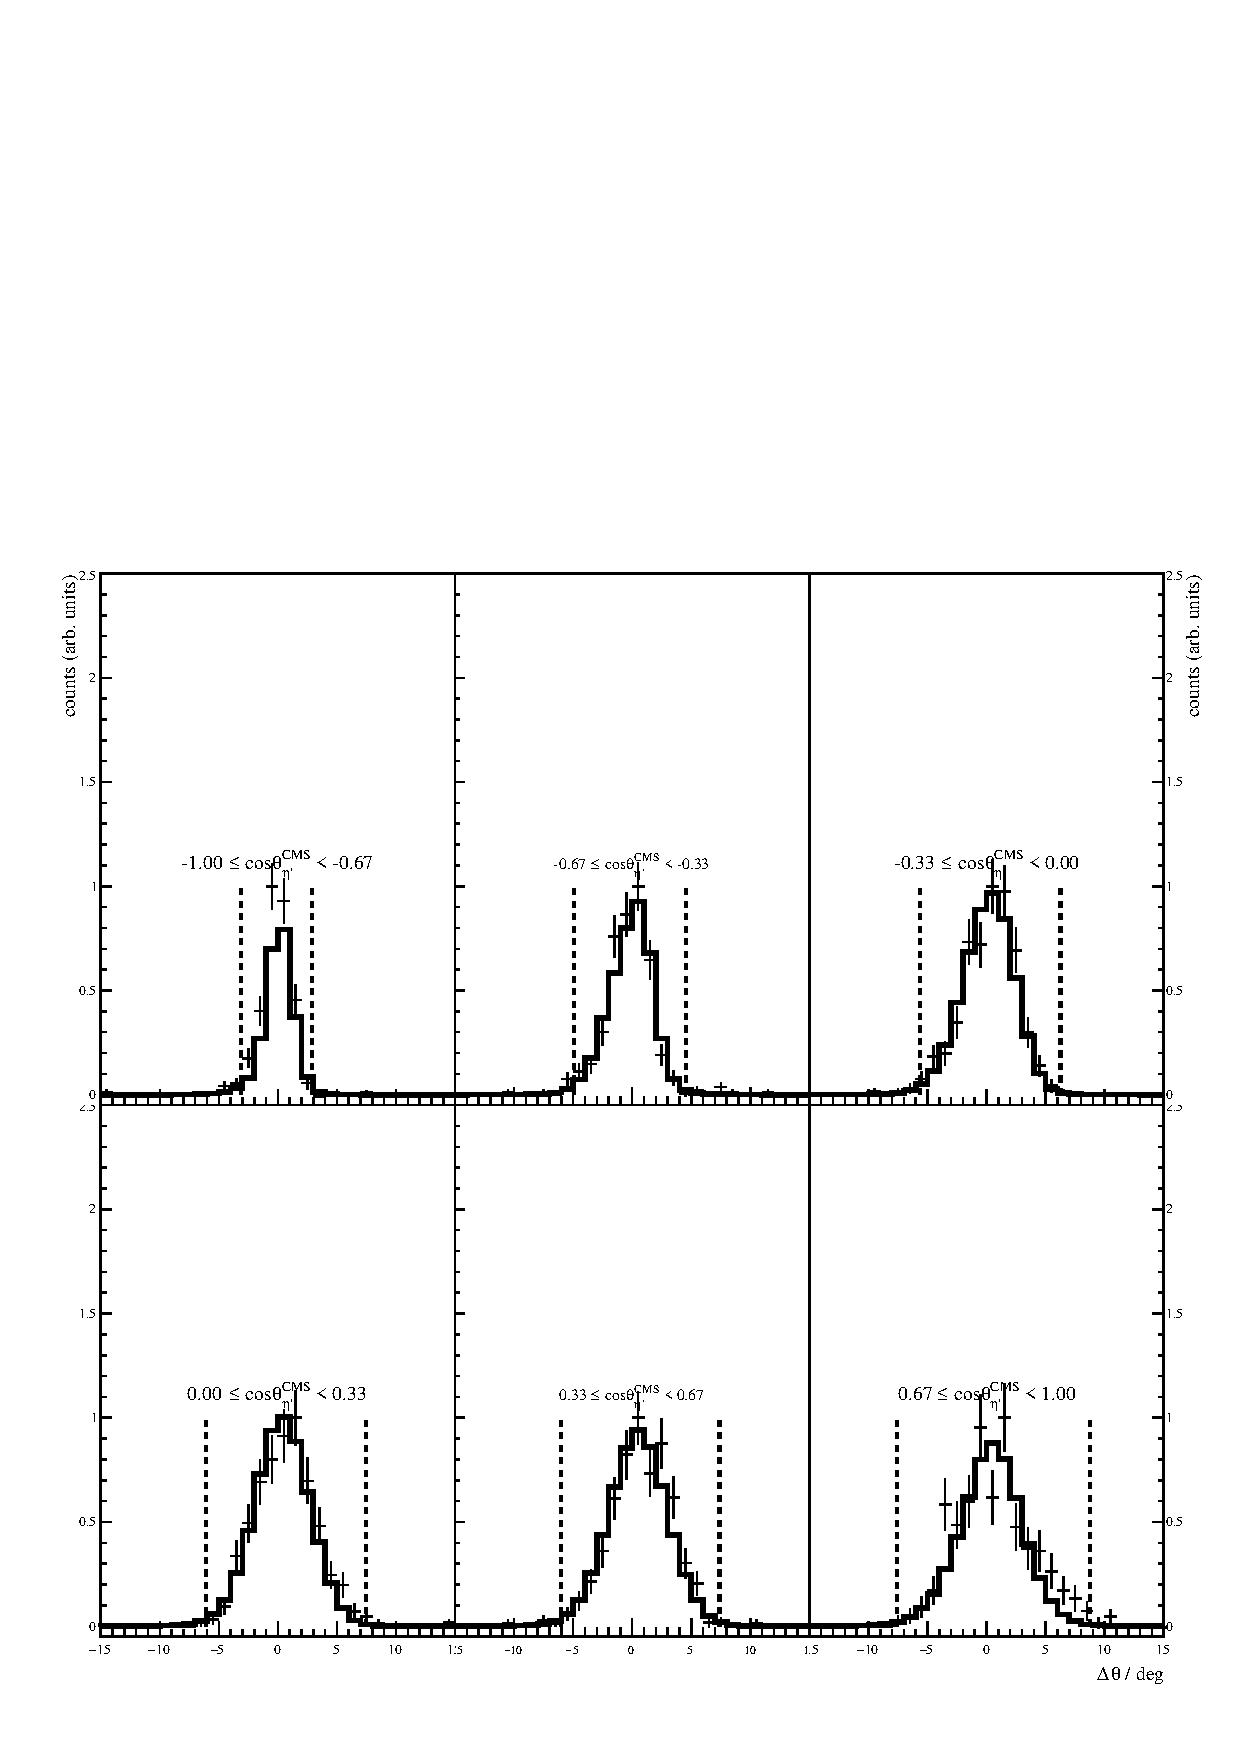
\includegraphics[width=\linewidth]{../figs/hydrogen/bin_cuts/thetacut_ebin1.pdf}
		\subcaption{$\SI{1500}{\mega\eV}\leq E_\gamma<\SI{1600}{\mega\eV}$}
	\end{subfigure}
	
	\begin{subfigure}{\linewidth}
		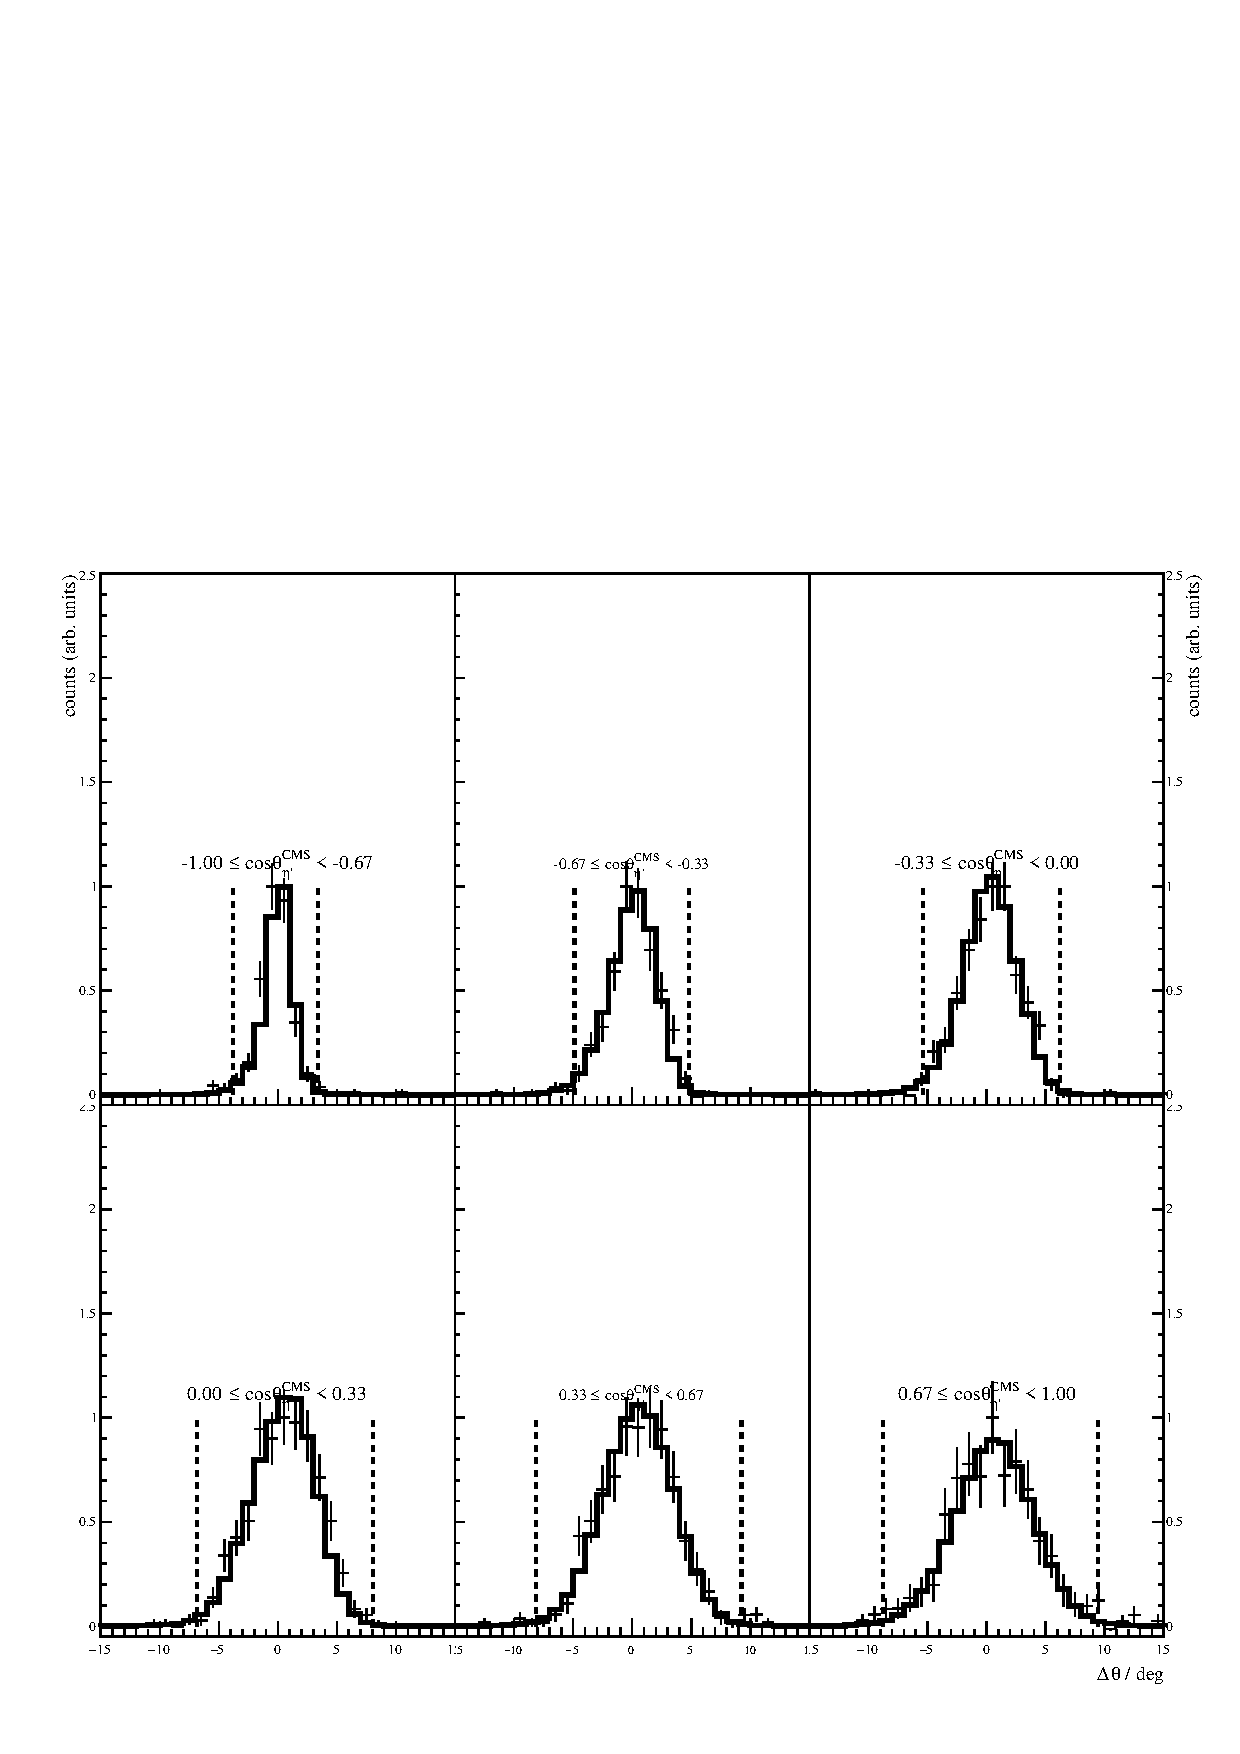
\includegraphics[width=\linewidth]{../figs/hydrogen/bin_cuts/thetacut_ebin2.pdf}
		\subcaption{$\SI{1600}{\mega\eV}\leq E_\gamma<\SI{1700}{\mega\eV}$}
	\end{subfigure}
\caption{Polar angle difference $\Delta\theta$ for all energy and angular bins. Data points are displayed as open circles, scaled Monte Carlo data belonging to $\eta'$ photoproduction is displayed as solid histogram. The determined cut ranges are indicated by the dashed red lines.}
\end{figure}
\begin{figure}[H]
	\ContinuedFloat
	\begin{subfigure}{\linewidth}
		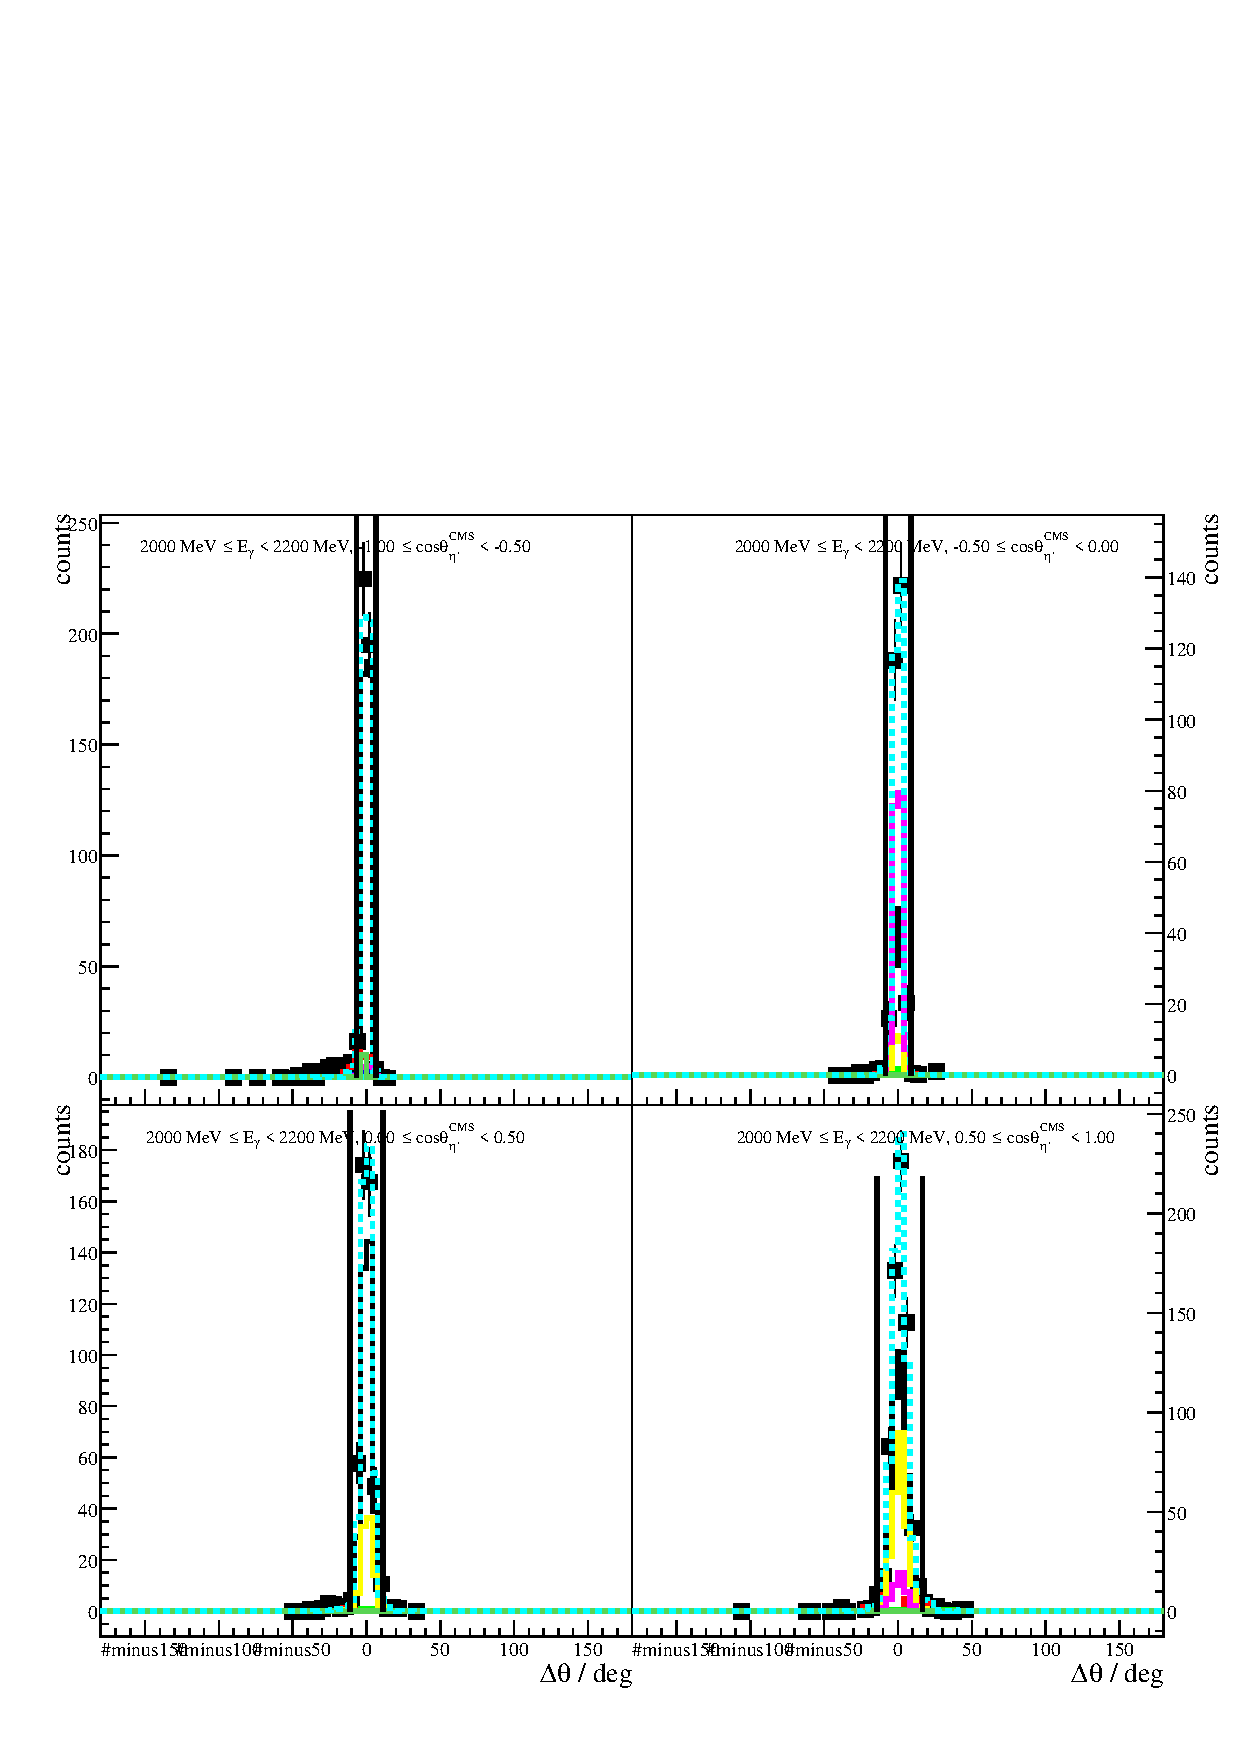
\includegraphics[width=\linewidth]{../figs/hydrogen/bin_cuts/thetacut_ebin3.pdf}
		\subcaption{$\SI{1700}{\mega\eV}\leq E_\gamma<\SI{1800}{\mega\eV}$}
	\end{subfigure}
\caption{Polar angle difference $\Delta\theta$ for all energy and angular bins. Data points are displayed as open circles, scaled Monte Carlo data belonging to $\eta'$ photoproduction is displayed as solid histogram. The determined cut ranges are indicated by the dashed red lines.}
\label{fig:apptheta}	
\end{figure}
Figure \ref{fig:apptheta} shows the polar angle difference for all energy and angular bins. Cut ranges were determined from a \textsc{Gaussian} fit to the data points. Only slight dependency on beam energy can be identified whereas clear correlation between width of the distribution and meson polar angle exists. This is due to the hit detectors which exhibit different angular resolutions, as has been discussed in the main part. Only $\eta'$ Monte Carlo data are fitted because the measured points do not give enough reference points for the fit to identify different contributing final states. There is good agreement between Monte Carlo simulations and measured data.
\newpage
\subsection{Missing mass}
\begin{figure}[H]
	\centering
	\begin{subfigure}{\linewidth}
		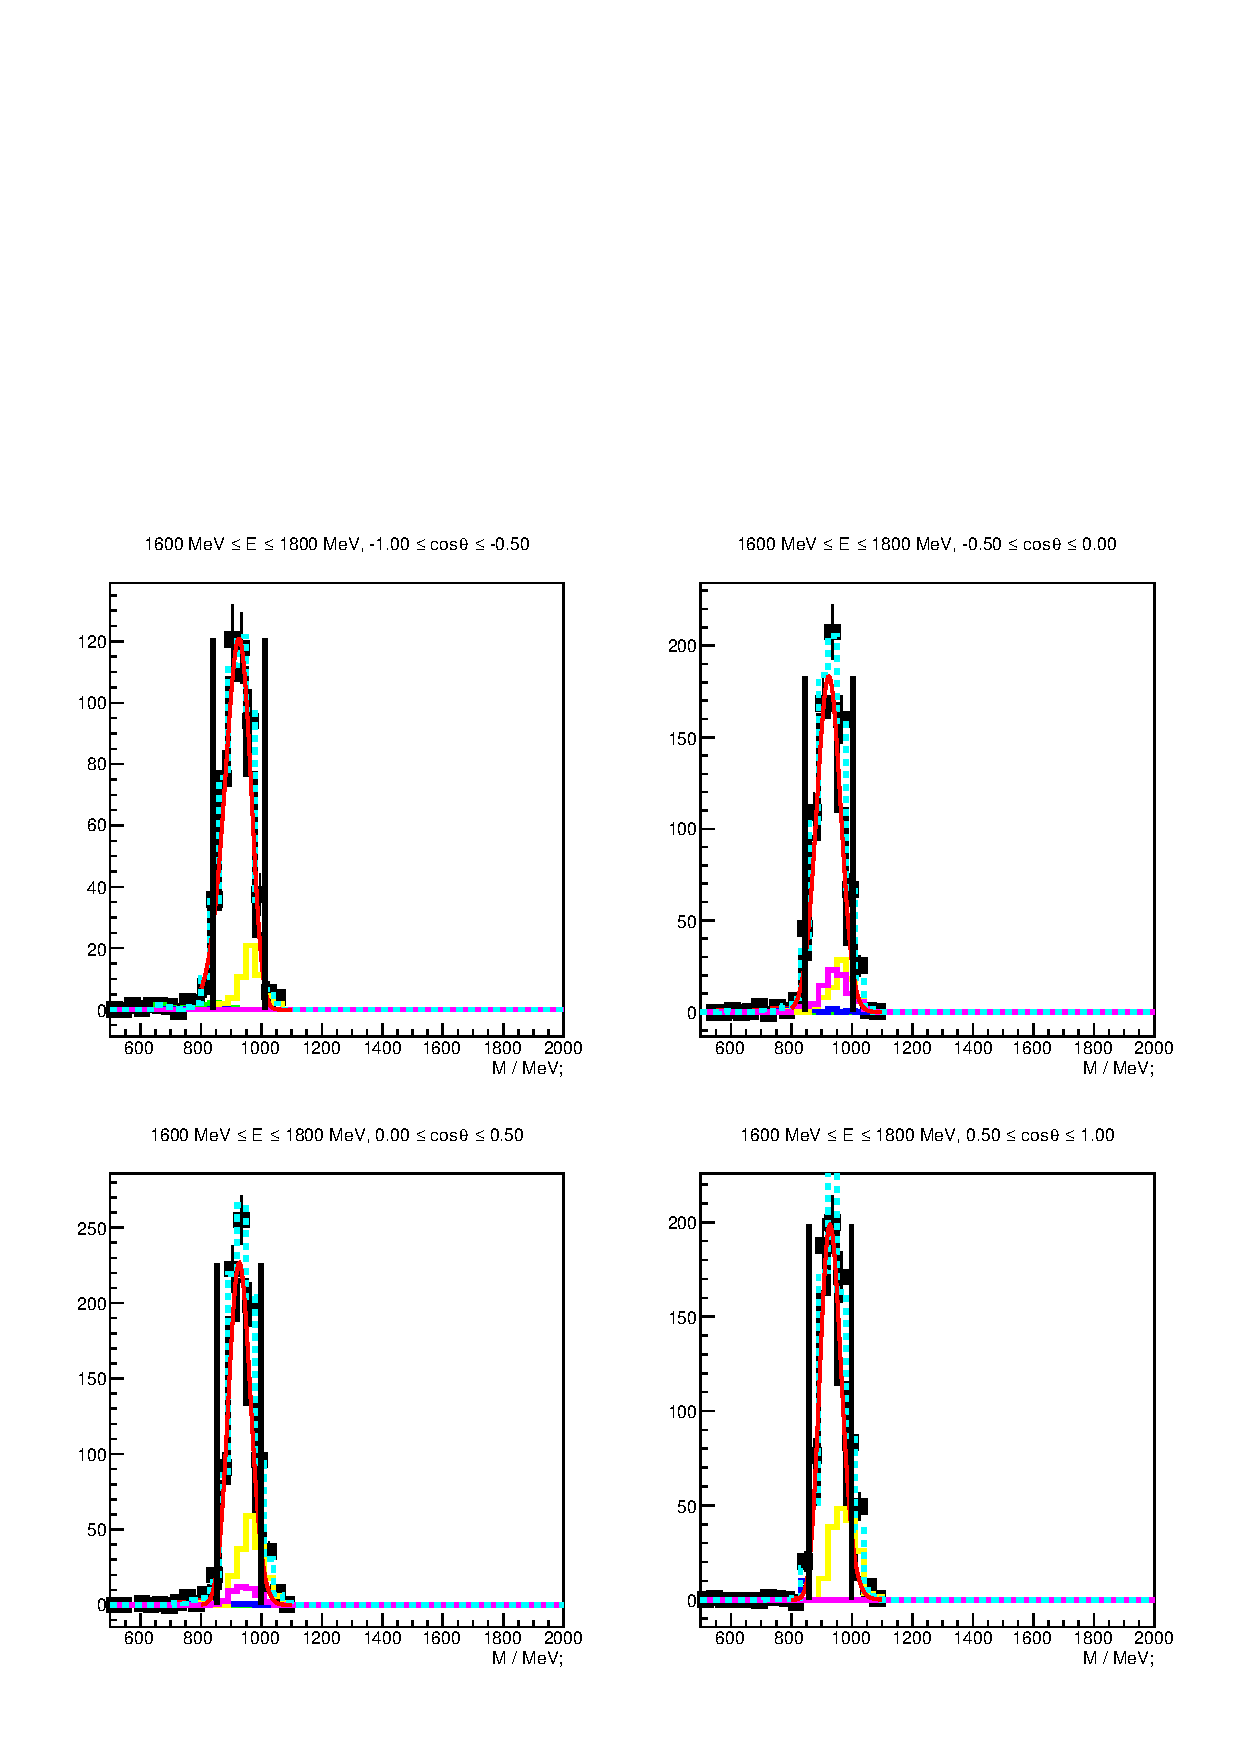
\includegraphics[width=\linewidth]{../figs/hydrogen/bin_cuts/mismcut_ebin1.pdf}
		\subcaption{$\SI{1500}{\mega\eV}\leq E_\gamma<\SI{1600}{\mega\eV}$}
	\end{subfigure}
	
	\begin{subfigure}{\linewidth}
		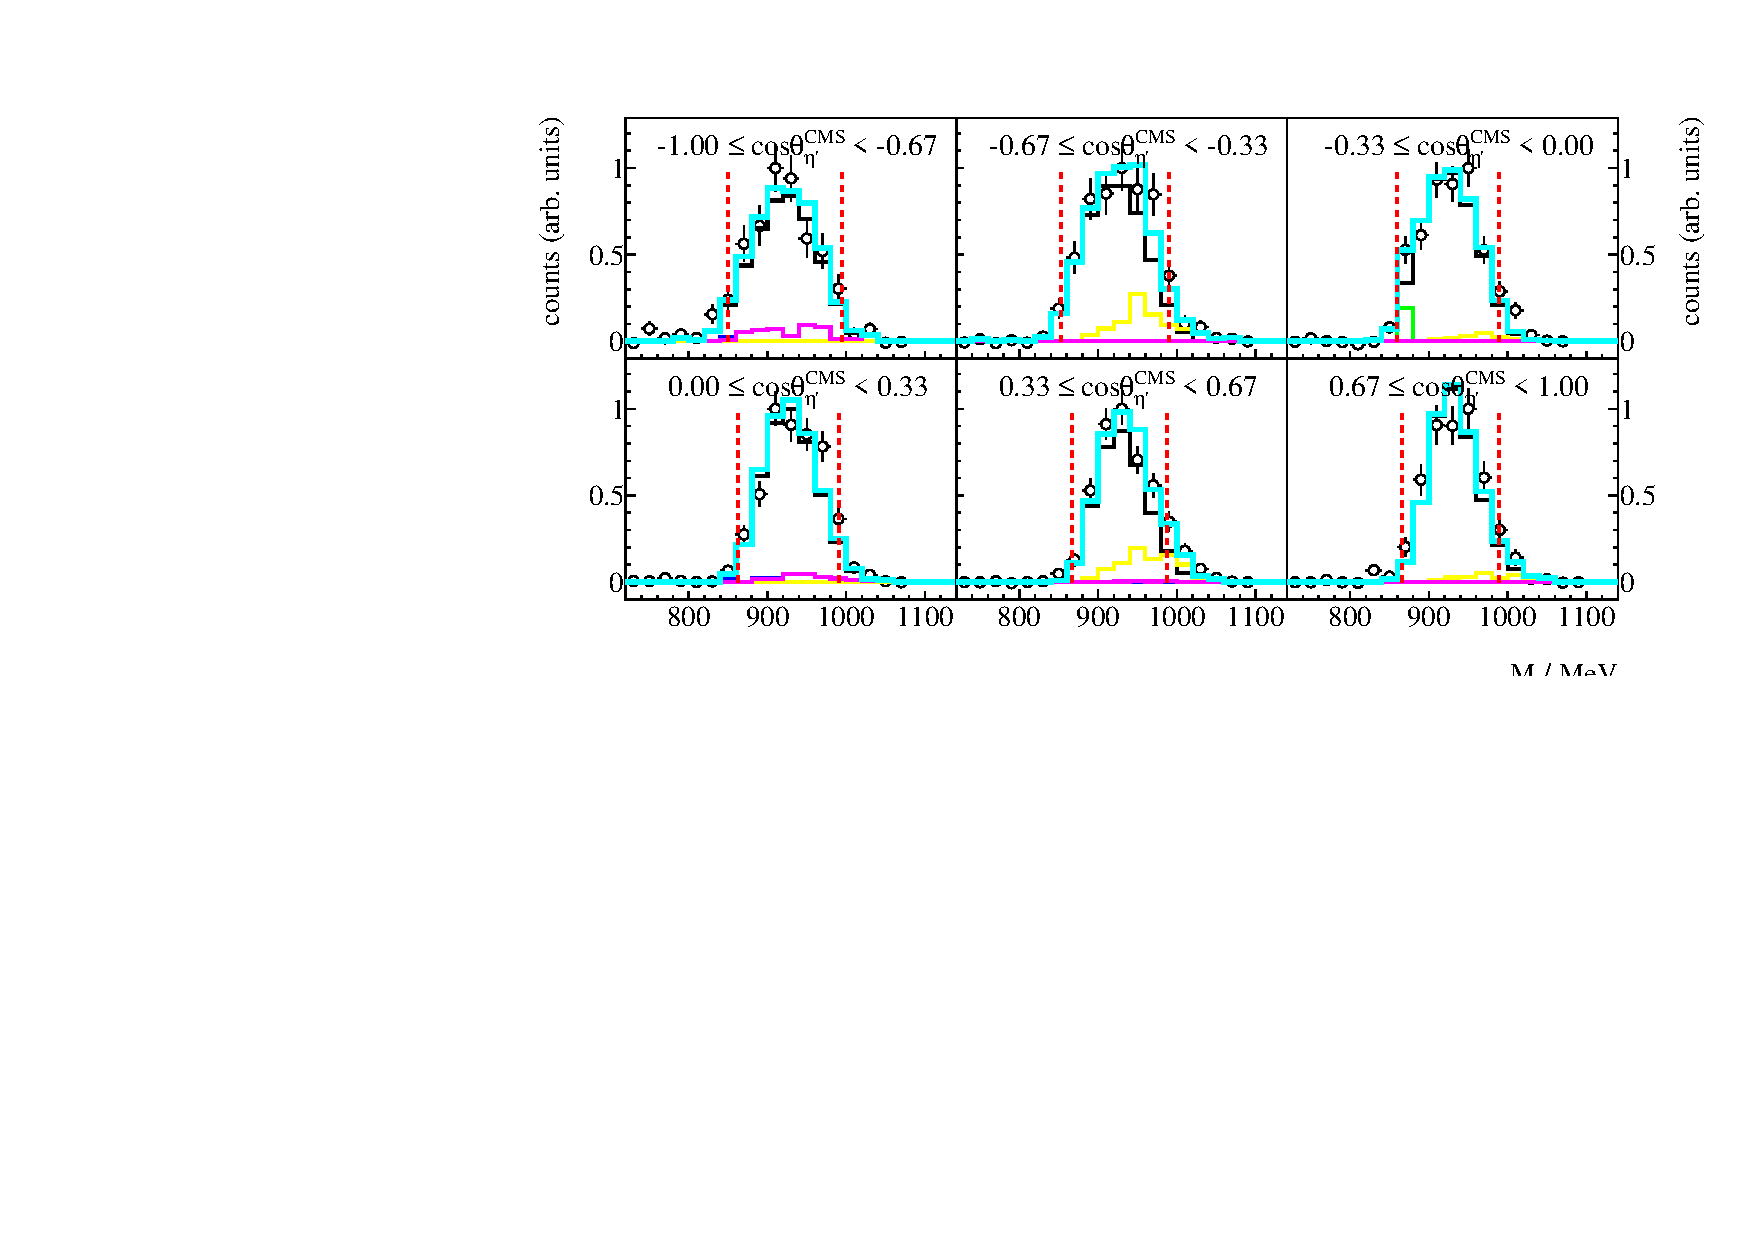
\includegraphics[width=\linewidth]{../figs/hydrogen/bin_cuts/mismcut_ebin2.pdf}
		\subcaption{$\SI{1600}{\mega\eV}\leq E_\gamma<\SI{1700}{\mega\eV}$}
	\end{subfigure}
\caption{Missing mass $m_x$ for all energy and angular bins. Data points are displayed as open circles, scaled Monte Carlo data belonging to $\eta'$ (black), $2\pi^0$ (yellow) and $\pi^0\eta$ (magenta) photoproduction is displayed as solid histogram while their sum is displayed as turquoise histogram. The determined cut ranges are indicated by the dashed red lines.}
\end{figure}
\begin{figure}[H]
	\ContinuedFloat
	\begin{subfigure}{\linewidth}
		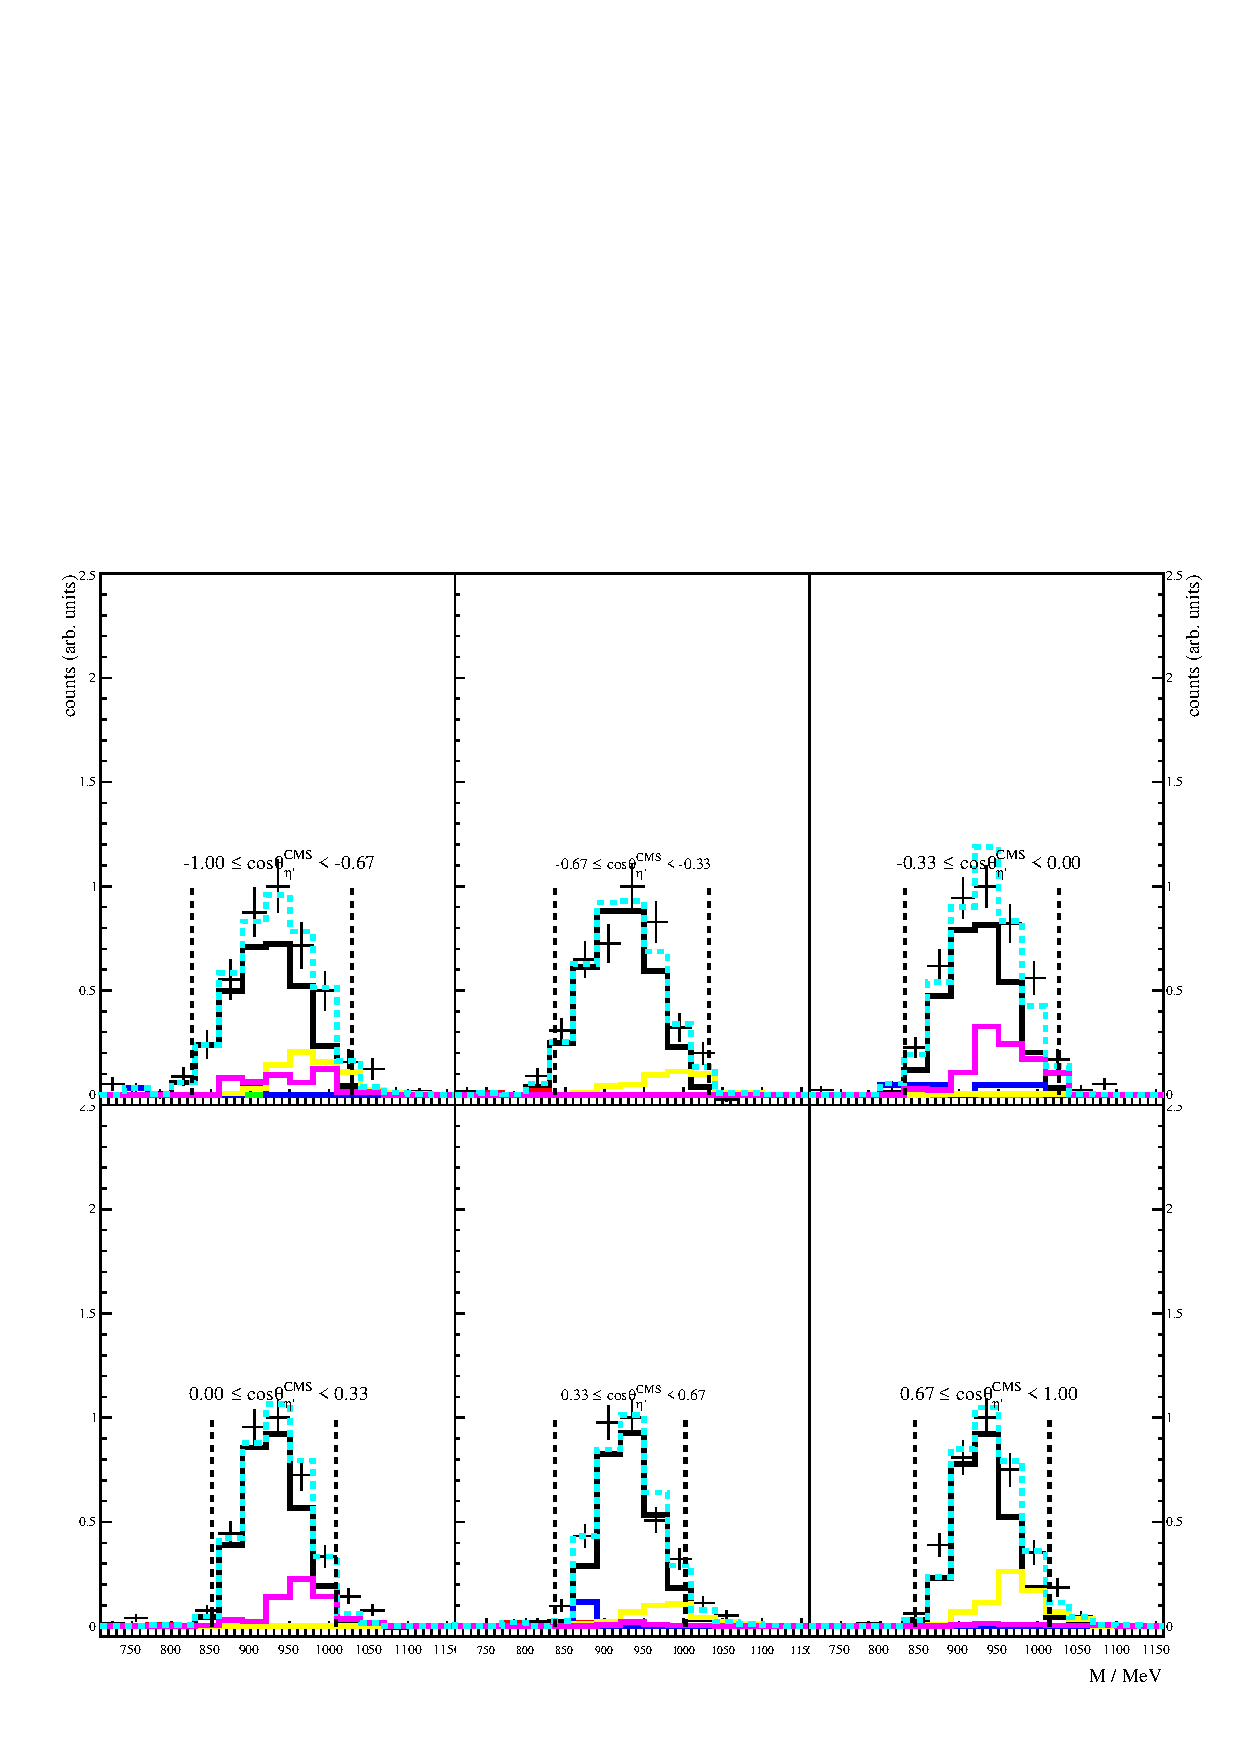
\includegraphics[width=\linewidth]{../figs/hydrogen/bin_cuts/mismcut_ebin3.pdf}
		\subcaption{$\SI{1700}{\mega\eV}\leq E_\gamma<\SI{1800}{\mega\eV}$}
	\end{subfigure}
	\caption{Missing mass $m_X$ for all energy and angular bins. Data points are displayed as open circles, scaled Monte Carlo data belonging to  $\eta'$ (black), $2\pi^0$ (yellow) and $\pi^0\eta$ (magenta) photoproduction is displayed as solid histogram while their sum is displayed as turquoise histogram. The determined cut ranges are indicated by the dashed red lines.}
	\label{fig:appmism}
\end{figure}
Figure \ref{fig:appmism} shows the missing mass for all energy and angular bins. Cut ranges were determined from a \textsc{Novosibirsk} fit to the Monte Carlo data. Only slight dependency on meson polar angle can be identified. Especially at higher beam energies the missing mass peak grows wider with flat background contributions from $2\pi^0$ and $\pi^0\eta$ production towards higher masses. The Monte Carlo fit mostly shows consistency with the fit of the invariant mass spectra. However, spectra are to be seen with caution, since the shapes of the two different background contributions are very similar and there is no other reference point in the missing mass spectrum as opposed to the invariant mass. Fits to the invariant mass spectra may reveal background contributions where a fit to the missing mass spectrum failed to find any. There is good agreement between Monte Carlo simulations and measured data.
\newpage
\subsection{Invariant mass}
\begin{figure}[H]
	\centering
	\begin{subfigure}{\linewidth}
		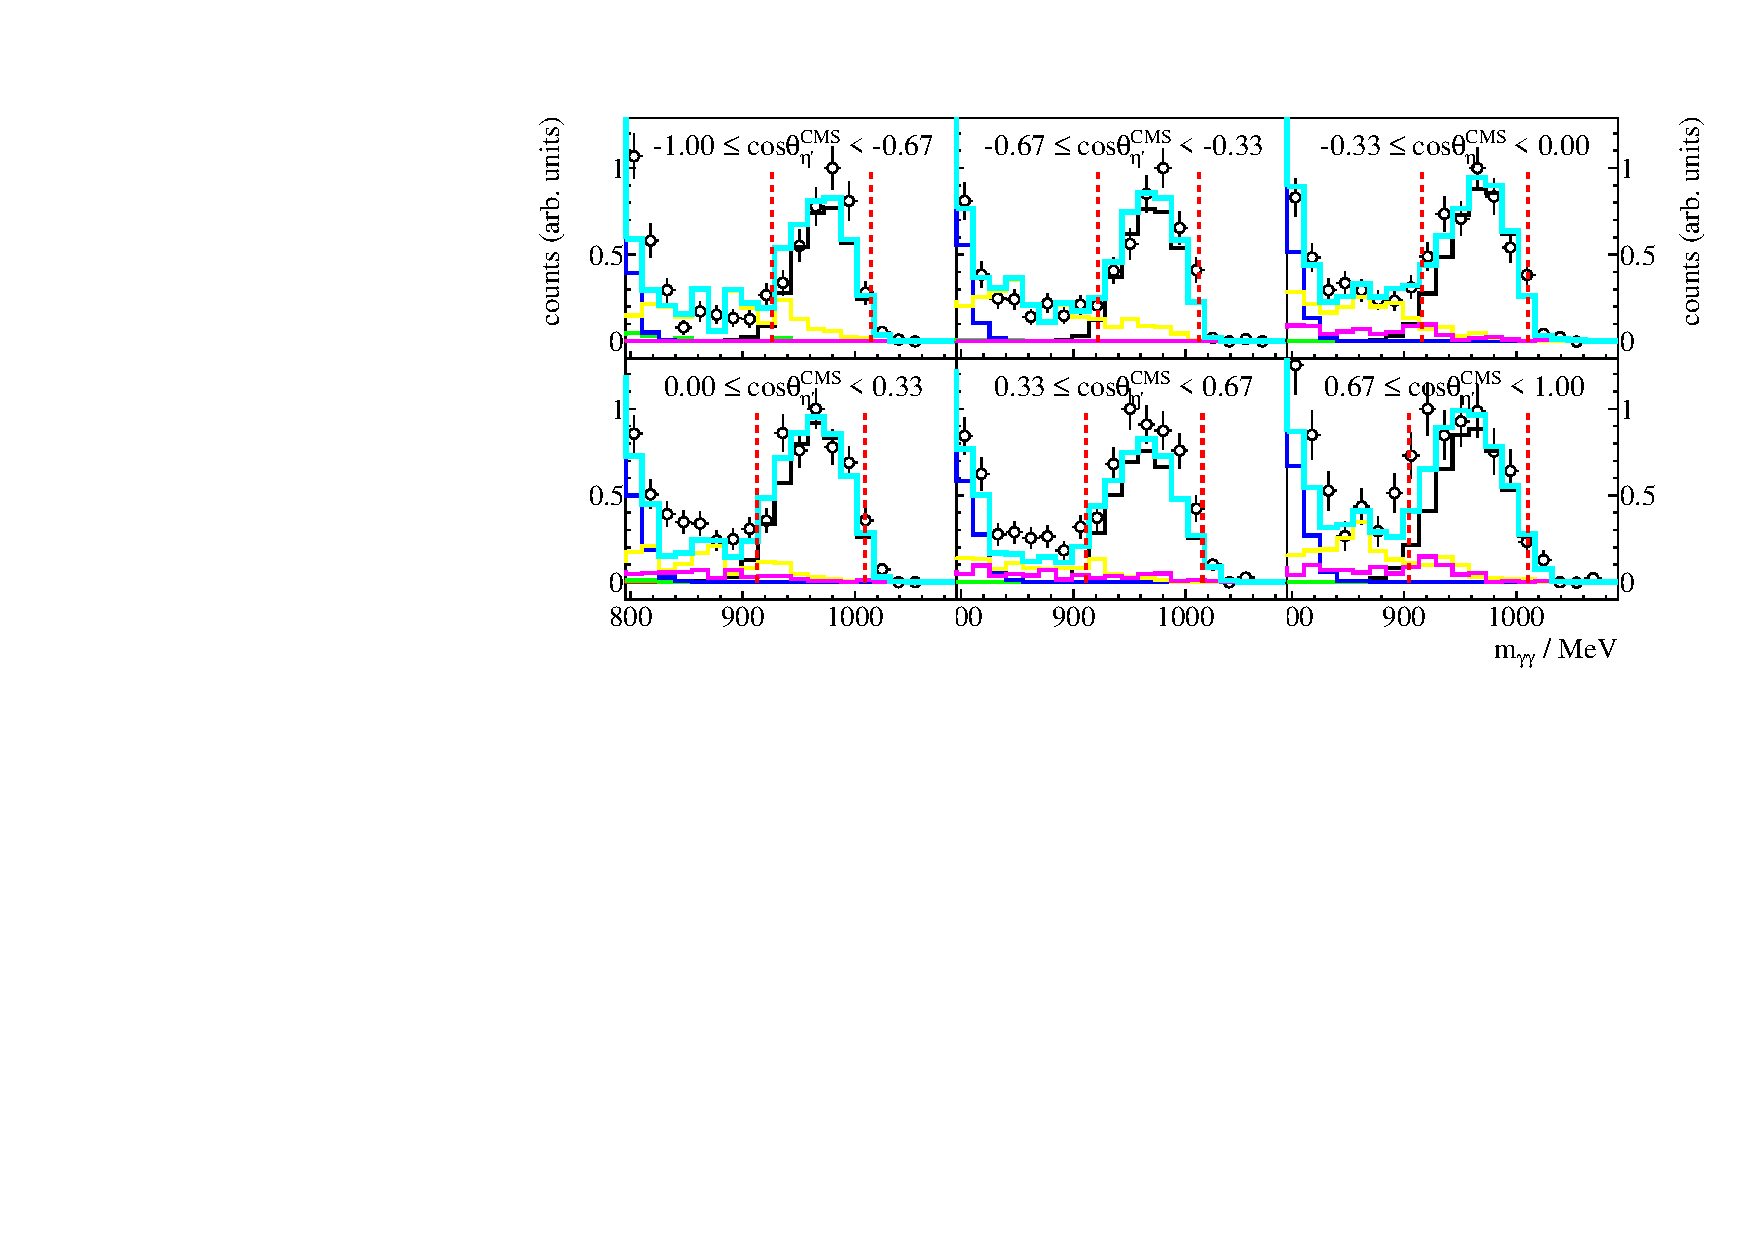
\includegraphics[width=\linewidth]{../figs/hydrogen/bin_cuts/invcut_ebin1.pdf}
		\subcaption{$\SI{1500}{\mega\eV}\leq E_\gamma<\SI{1600}{\mega\eV}$}
	\end{subfigure}
	
	\begin{subfigure}{\linewidth}
		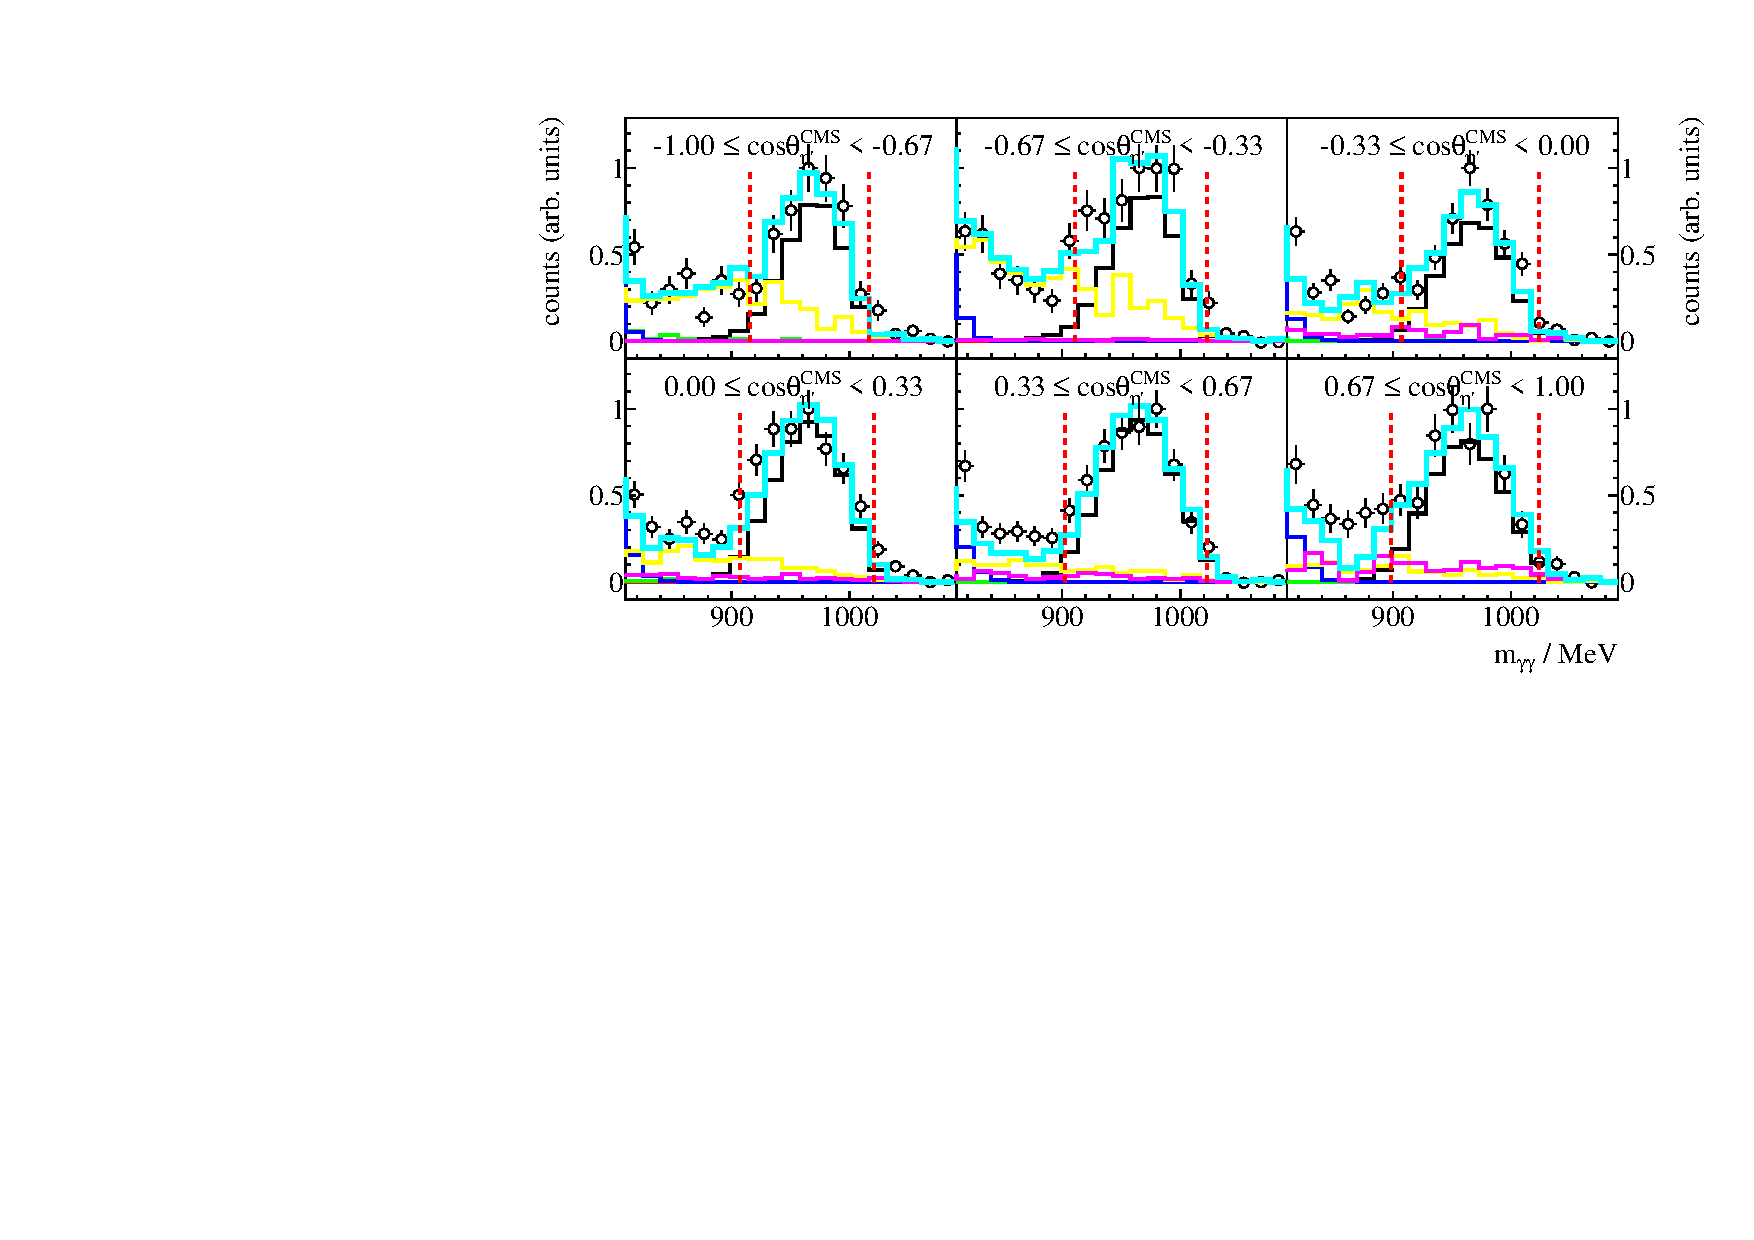
\includegraphics[width=\linewidth]{../figs/hydrogen/bin_cuts/invcut_ebin2.pdf}
		\subcaption{$\SI{1600}{\mega\eV}\leq E_\gamma<\SI{1700}{\mega\eV}$}
	\end{subfigure}
\caption{Invariant mass $m_\text{meson}$ for all energy and angular bins. Data points are displayed as open circles, scaled Monte Carlo data belonging to $\eta'$ (black), $2\pi^0$ (yellow), $\pi^0\eta$ (magenta), $\pi^0$ (green) and $\omega$ (blue) photoproduction is displayed as solid histogram while their sum is displayed as turquoise histogram. The determined cut ranges are indicated by the dashed red lines.}
\end{figure}
\begin{figure}[H]
	\ContinuedFloat
	\begin{subfigure}{\linewidth}
		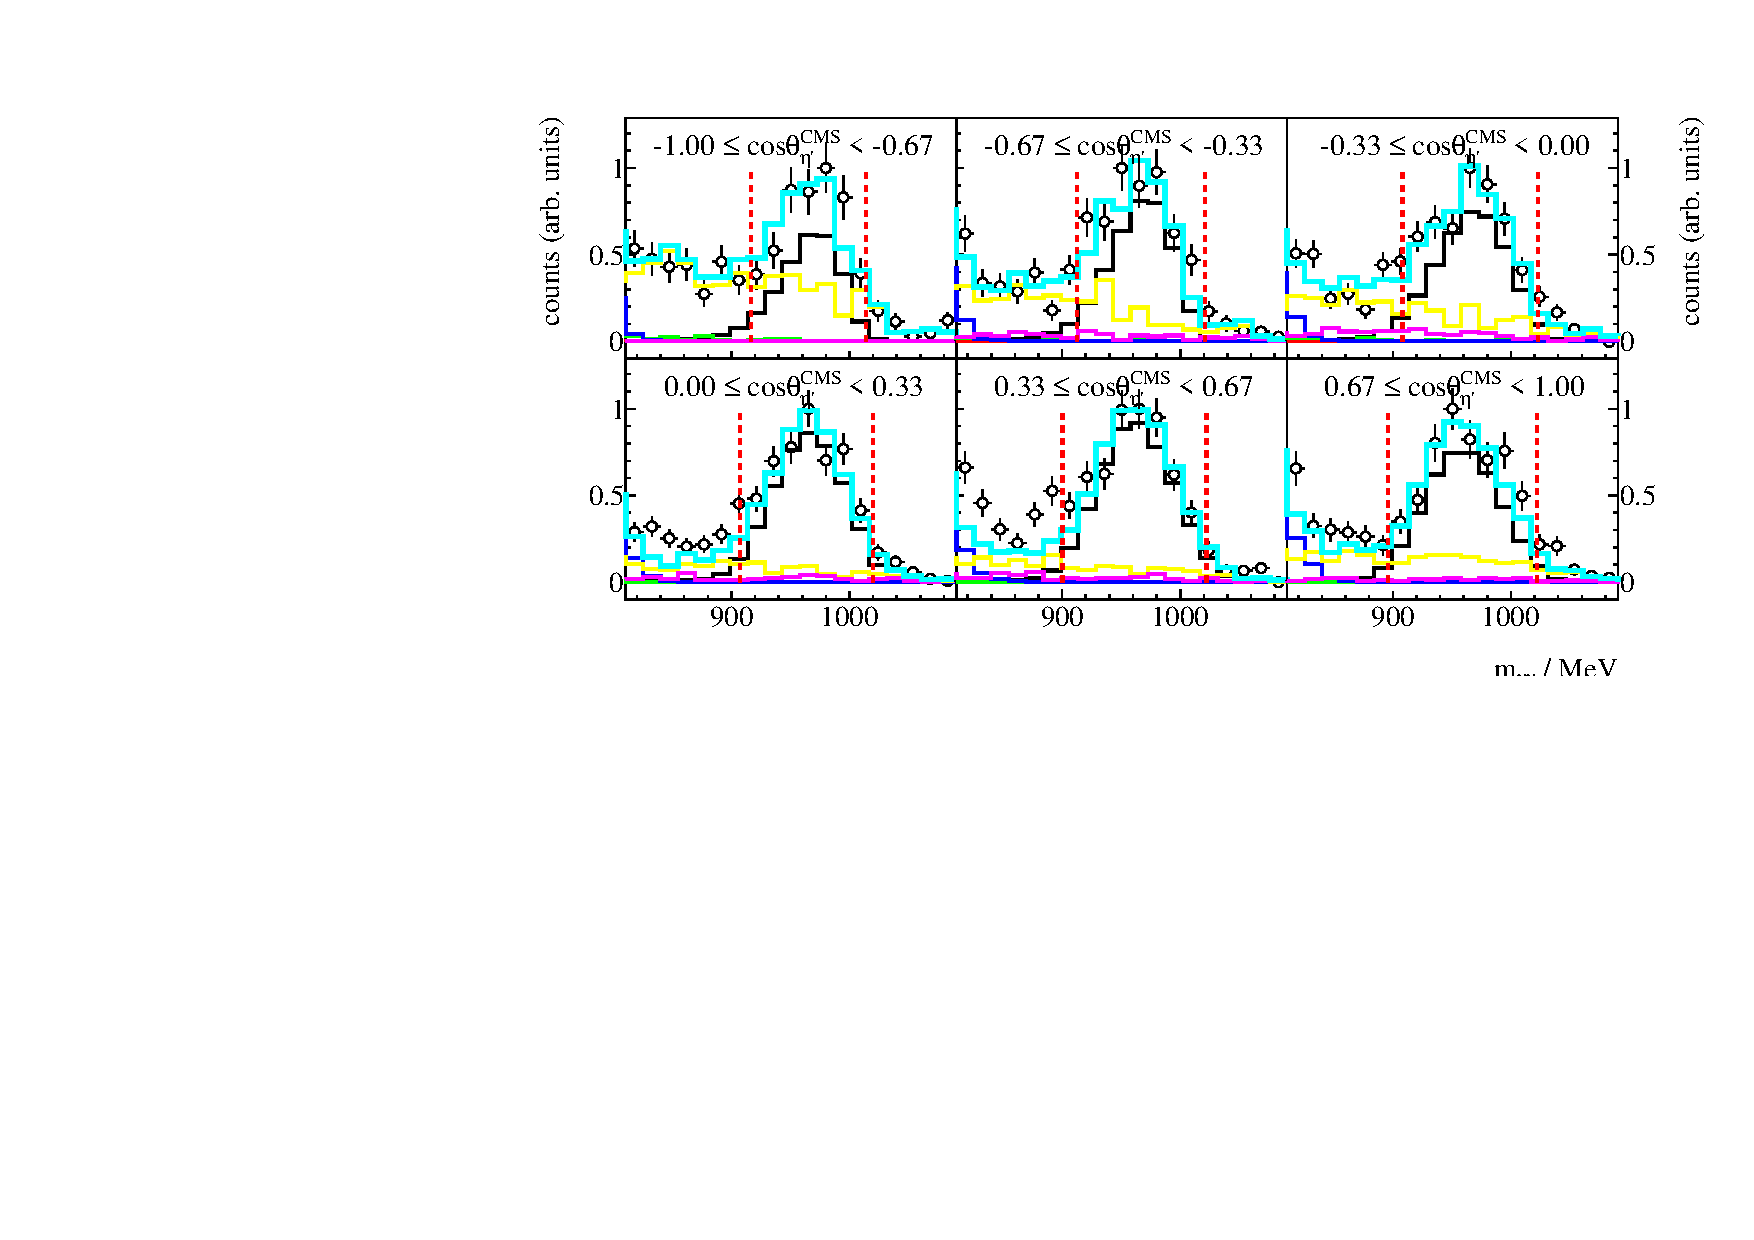
\includegraphics[width=\linewidth]{../figs/hydrogen/bin_cuts/invcut_ebin3.pdf}
		\subcaption{$\SI{1700}{\mega\eV}\leq E_\gamma<\SI{1800}{\mega\eV}$}
	\end{subfigure}
\caption{Invariant mass $m_\text{meson}$ for all energy and angular bins. Data points are displayed as open circles, scaled Monte Carlo data belonging to $\eta'$ (black), $2\pi^0$ (yellow), $\pi^0\eta$ (magenta), $\pi^0$ (green) and $\omega$ (blue) photoproduction is displayed as solid histogram while their sum is displayed as turquoise histogram. The determined cut ranges are indicated by the dashed red lines.}
\label{fig:appinv}
\end{figure}
Figure \ref{fig:appinv} shows the invariant mass for all kinematic bins. Hardly any dependence on meson direction and beam energy is observed. However, background contributions are especially observed in very forward and backward direction towards higher beam energies in consistency with findings from the missing mass spectra.  A flat background is realized by $2\pi^0$ and $\pi^0\eta$ production. There is good agreement between Monte Carlo simulations and measured data.
\chapter{Discussion of binned fits}
\label{app:binnedfits}
Investigation of toy Monte Carlo experiments (cf. section \ref{sec:sigma_etap}) revealed that the choice of binning leads to systematic errors regarding the parameter $\Sigma$ when fitting a binned distribution to the equation 
\begin{equation}
	A\left(\phi\right)=\Sigma\cdot\cos\left(2\left(\alpha^\parallel-\phi\right)\right).
\end{equation}
To investigate this further, the distributions $A\left(\phi\right)$ from different toy Monte Carlo experiments where fitted for several binnings in $\phi$. Three different Monte Carlo experiments were considered, each corresponding roughly to the expected statistics in one kinematic bin for $\pi^0$, $\eta$ and $\eta'$ photoproduction, respectively. For simplicity's sake, only least squares fits are shown here, although similar results were found for \textsc{Bayesian} fits also. The equivalency of \textsc{Bayesian} and least squares fit has been demonstrated sufficiently up until now. To identify the bias that is introduced by binning the data, 10000 toy Monte Carlo bins for each setting are fitted for $n=10,15,20,\dots,100$ bins. Then the dependence from the amount of bins of the mean $\mu$ of the normalized residuals $\xi$ as well as the mean $\chi^2$ value of all fits is investigated.
\chapter{Investigation of posteriors without truncation}
\label{app:trunc}
In section \ref{sec:sigma_etap} the investigation of posterior distributions from unbinned \textsc{Bayesian} fits was incomplete, since the normalized residuals as well as the likelihood pool could not be built with truncated posteriors. This is now supplemented here. After the fits have been repeated without implementing a truncation for the posteriors, all introduced measures to argue good fit quality can be examined.